
\color{Emerald}

      \providecommand{\cmm}{\textrm{,}}
      
    \begin{figure}[ht]
  \centering
  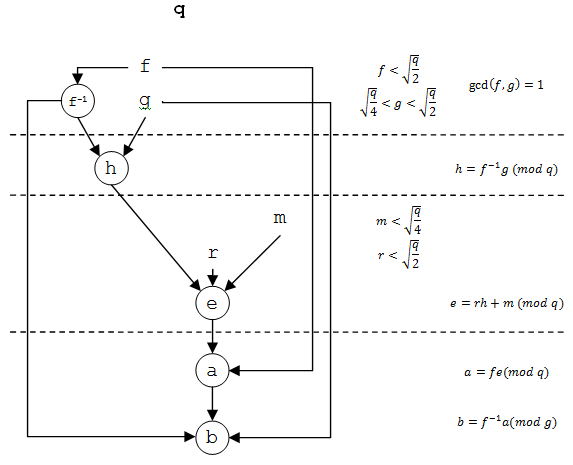
\includegraphics[scale=0.8]{share/congruental.png}
  \caption{Схема конгруентной криптосистемы}
  \label{fig:congruental}
\end{figure}

	
    \vspace{8mm}Когруэнтая криптосистема описана в \cite{HoffsteinIntroduction-08}.\par Конгруэнтная криптосистема очень удобна, как начальная модель для рассмотрения. Ее запись можно свести к функции получения расшифрованного сообщения в следующей форме:
    \[\pi^*=f\left(\pi \cmm r\cmm q\cmm {\textrm f}\cmm g\right)\cmm \begin{cases}\pi\cmm r\cmm q\cmm {\textrm f}\cmm g\in{\mathbb Z}\\g<q\cmm {\textrm f}<\sqrt{q/2}\\\exists\ {\textrm f}^{-1}\ mod\ q={\textrm f}^{-1}_q\\gcd(f\cmm g)=1\end{cases}\]
    
    \begin{multline*}
        \pi^*=\left(f^{-1}_g\cdot\left({\textrm f}\cdot\psi\ mod\ q\right)\right)\ mod\ g
        =\left({\textrm f}^{-1}_g\cdot\left({\textrm f}\cdot\left(r\cdot h+\pi \right)\ mod\ q\right)\right)\ mod\ g
        =\\=\left({\textrm f}^{-1}_g\cdot \left({\textrm f}\cdot\left(r\cdot\left(g\cdot{\textrm f}^{-1}_q\right)+\pi\right)\ mod\ q\right)\right)\ mod\ g
        ;
    \end{multline*}
    , где $\psi$ -- шифртекст, $\pi$ -- сообщение, $r$ -- случайное число, $q$, $g$, $f$ - параметры системы. Учитывая секретный и публичный ключи, соответственно, равенство можно перезаписать, как:
    \[pk=\left(g\cdot{\textrm f}^{-1}_q\cmm q\right)=\left(h\cmm q\right)\cmm \ sk=\left({\textrm f}\cmm g\right)\]
    \begin{align*}\everybeforeautobreak{=}\begin{autobreak}
        \pi^*
        =\left(f\left(sk\right)\cdot\left(sk_1\cdot \left(r\cdot pk_1+\pi \right)\ mod\ pk_2\right)\right)\ mod\ sk_2
        =f\left(\left(r\cdot pk_1+\pi \right)\cmm pk_2\cmm sk\cmm sk_1\cmm sk_2\right)
        =f\left(f\left(r\cdot pk_1\cmm \pi \right)\cmm pk_2\cmm sk\cmm sk_1\cmm sk_2\right)
        =f\left(f\left(\pi \cmm f(r\cmm pk_1)\right)\cmm pk_2\cmm sk\cmm sk_1\cmm sk_2\right)
        =\left(f(\pi \cmm u)~mod\ pk_2\right)~mod\ sk_2
    \end{autobreak}\end{align*}
    
    Наличие публичного и секретного ключа позволяет реализовать систему асимметричной криптографии. К обеим формам записи мы будем приходить, рассматривая и последующие криптосистемы. Такие нотации удобны, так как они показывают ``уровневую'' структуру криптографических схем, где каждый этап работы соответствует одному или нескольким порядкам оператора приоритета (т. е. скобок). Первая форма описывает криптосистему, раскрывая содержание её параметров на уровне математической записи, в то время как вторая форма описывает более высокий уровень абстракции, раскрывающий содержание криптографической схемы или протокола. Груба говоря, первая форма - эта форма математических примитивов, а вторая форма - это форма криптографических примитивов.\textbf{}
    
    Для конгруэнтной криптосистемы вторую форму записи можно обобщить, как:
    \begin{align*}\everybeforeautobreak{=}\begin{autobreak}
        \pi^*=\psi~mod\ sk_2
        =\left(t~mod\ pk_2\right)~mod\ sk_2
        =\left(f(\pi \cmm u)~mod\ pk_2\right)~mod\ sk_2
        =\left(f(\pi \cmm f(r\cmm pk_1))~mod\ pk_2\right)~mod\ sk_2
    \end{autobreak}\end{align*}
    , где $\pi \in \Pi$ - элемент множества открытого текста, $u\in U$ - элемент шумового множества, $r\in R$ - элемент множества случайных значений, $t\in T$ - элемент множества усеченного (редуцированного) шифртекста, $\psi \in \Psi $ - элемент множества шифртекста.
    
    Эта третья форма записи является более специфичной и отображает некоторые преобразования, которые производятся над исходным сообщением. В-частности имеет место следующая карта отображений:
    \[\left. \begin{array}{c}
    \Pi  \\ 
    {\textrm R}\to {\textrm U} \end{array}
    \right\}\to {\textrm T}\to \Psi \] 
    \[\Pi \to (\Pi {\textrm +}pk_1\cdot {\textrm R}={\textrm T)}\to \Psi \] 

    Покажем на примере конгруэнтной криптосистемы, каким образом её можно ее дополнить, чтобы производить вычисления над зашифрованными сообщениями.
    Для полей целых чисел при паре взаимно простых значений $pk_1$ и $sk_2$ операции умножения и сложения над шифртекстом реализуют гомоморфизм для всех изоморфных пространств, позволяя определить операции над шифртекстом как обобщенные:
    \begin{align*}\everybeforeautobreak{=}\begin{autobreak}
      \psi_1+\psi_2
      =\left(\left({\pi }_1+g\cdot r_1\right)+\left({\pi }_2+g\cdot r_2\right)\right)\ mod\ q
      =\left({\pi }_1+g\cdot r_1+q\cdot k\right)+\left({\pi }_1+g\cdot r_2+q\cdot k\right)
      =\left({\pi }_1+{\pi }_2\right)+g\cdot \left(r_1+r_2\right)+q\cdot 2k
      =\left(\left({\pi }_1+{\pi }_2\right)+g\cdot \left(r_1+r_2\right)\right){\textrm \ }mod\ q
    \end{autobreak}\end{align*}

    \small
    \begin{dmath*}
    \psi_1 \times \psi_2
      ={\psi }_1\cdot {\psi }_2=\left({\pi }_1+g\cdot r_1\right)\cdot \left({\pi }_2+g\cdot r_2\right)\ mod\ q
      =\left({\pi }_1+g\cdot r_1+q\cdot k\right)\cdot \left({\pi }_2+g\cdot r_2+q\cdot k\right)
      ={\pi }_1\cdot {\pi }_2+g\cdot {\pi }_1\cdot r_2+q\cdot {\pi }_1\cdot k+g\cdot {\pi }_2\cdot r_1+g\cdot g\cdot r_1r_2+q\cdot g\cdot r_1k+q\cdot {\pi }_2\cdot k+q\cdot g\cdot kr_2+q\cdot q\cdot k^2
      ={\pi }_1\cdot {\pi }_2+g\cdot {\pi }_1\cdot r_2+g\cdot {\pi }_2\cdot r_1+g\cdot g\cdot r_1r_2+q\cdot {\pi }_1\cdot k+q\cdot {\pi }_2\cdot k+q\cdot g\cdot kr_1+q\cdot g\cdot kr_2+q\cdot q\cdot k^2
      =\left({\pi }_1\cdot {\pi }_2+g\cdot {\pi }_1\cdot r_2+g\cdot {\pi }_2\cdot r_1+g\cdot g\cdot r_1r_2\right)\ mod\ q=\left({\pi }_1\cdot {\pi }_2+g\cdot \left({\pi }_1\cdot r_2+{\pi }_2\cdot r_1+g\cdot r_1r_2\right)\right)\ mod\ q
    \end{dmath*}
    \normalsize

    Как видно, результаты аддитивной и мультипликативной операций обладают той же формой, что и исходные шифртексты. Из-за монотонно возрастающего значения $r$, обе операции ведут к накоплению ошибки в пространстве шифртекста. Операции выполняются, пока $\pi $ не превысит значение $g$ и $t=\pi +g\cdot r$  не превысит значение $q$. Это можно записать как набор условий для функции вычислений $C$:
    \[C\left({\psi }_1\cmm \psi_2\cmm \dots \cmm {\psi }_n\right)\to {\psi }_C\cmm ~{\pi }_C<g\cmm ~{\pi }_C+g\cdot r_C<q\] 
    
    Таким образом, мы можем говорить о некоторой глубине вычислений по сложению и умножению. Однако, точное определение этого понятия, а также количественная оценка несколько затруднительны, при наличии сразу двух независимых условий. Для упрощения можно использовать понятие глубины вычислений с нулевым шумом ($r_C=0$), глубине вычислений по шуму (${\pi }_C=0$), а также глубине вычислений с нормированными шифртекстом и шумом ($\forall {\pi }_{1..n}:\pi =1\ или\ \forall r_{1..n}:r=1$), которое выражается в минимальном количестве операций, которые может выдержать цепочка вычислений $C$.
    Кроме этого, также можно использовать отношение мощности множеств:
    \[\left|\Pi \right|<\frac{|{\textrm U}|}{|{\textrm R|}} \cmm \ \left|{\textrm T}\right|{\textrm <}|\Psi |\]
    
    Последний вариант представляется наиболее подходящим для оценки глубины вычислений, в особенности, если мощности множеств $\Pi $, ${\textrm R}$ и ${\textrm T}$ могут быть выражены друг через друга. Например, если мощности множеств можно получить через публичный и секретный ключи, и эти ключи имеют взаимосвязь, тогда, приняв во внимание, что для повышения криптостойкости за счёт введения вероятностной величины обычно выполняется условие $\left|\Pi \right|\ll |{\textrm U}|$, мы можем производить оценку глубины вычислений, рассматривая соотношения мощности шумового множества к множеству шифртекста.
    Также, оценка глубины вычислений и реализация гомоморфных операций вообще может усложняться в случае негенерализированных операций, так как производные продукты вычислений будут приводить к ещё большему накоплению ошибки. Сами же генерализированные операции представляются лучшим случаем для реализации гомоморфных систем, и, по возможности, в дальнейшем мы будем предполагать именно такие операции и оценивать на их основе глубину вычислений.
    Таким образом, на основе трёх представленных форм записи, мы можем рассматривать математические свойства, определяющие возможность гомоморфных операций, и криптографические свойства, которые эти операции реализуют. Третья форма записи позволяет рассмотреть общий параметр, связывающий криптографические и гомоморфных свойства системы. В этом плане выбор математического примитивна определяет накопление ошибки в пространстве шифртекста, в том время, как реализация криптографической схемы задаёт некоторый объём, который может выдержать эта ошибка.
    В основе классической NTRU заложены принципы конгруэнтной криптосистемы. Несмотря на то, что она изначально не использует элементы решетчатых пространств, оценку криптостойкости такой системы можно свести к задаче нахождения кратчайчешго вектора для двумерной векторной решётки.

    \color{Blue}
    Криптосистема Джентри, как и другие системы на решетках, может быть сведена к конгруэнтной криптосистеме.
    Функция шифрования записывается в виде:
    
    \[\psi \leftarrow {\pi }^*~mod\ B^{pk}_J\] 
    
    Функция расшифровки может быть представлена в виде:
    
    \[\pi \leftarrow \left(\psi ~mod\ B^{sk}_J\right)~mod\ B_I\] 
    
    Как видно для шифрования используется один уровень отображения, в то время как для расшифрования используется два отображения. Базис $B_I$ одновременно включает в себя и случайную составляющую, которая может быть описана распределением $D$:
    
    \[{\pi }^*\leftarrow Samp\left(B_I\cmm D\cmm r'\cmm {\pi }'\right);;\ {\pi }'\cmm r'\in {\mathbb Z}\] 
    
    Базисы $B_I$ и $B_J$ являются взаимно простыми.
    
    Базовую криптосистему Джентри в соответствии с нашей нотацией можно представить в виде:\textit{}
    
    \[{\pi }^*=\Psi ~mod\ B_I=\left(R~mod\ B^{sk}_J\right)~mod\ B_I=\left(\left(\pi ~mod\ B^{pk}_J\right)~mod\ B^{sk}_J\right)~mod\ B_I\] 
    
    В сравнении с записью конгруэнтной криптосистемы, там также можно выделить три уровня. С помощью различных базисов $B_J$ реализуется асимметричная криптосистема. В криптосистеме Джентри первую и вторую записи можно объединить в одну.
    
    Для построения своей криптосистемы Джентри использует ``решечатые'' пространства в полной мере, а ее криптоанализ, как и в случае с конгруэнтной криптосистемой, можно свести к задаче нахождения кратчайшего вектора. Принимая во внимание общую запись в нашей нотации, это показывает не только то, что криптосистема Джентри является обобщением конгруэнтной криптосисистемы, а конгруэнтная криптосистема является частным случаем криптосистемы Джентри на случай редуцирования размерности ``решетчатого'' пространства, но и анализ тех частей, из которых она состоит. Для построения такой криптосистемы используется пространство решеток и алгебра над полем идеалов. Причем, нет явной связи между этими двумя частями, что позволяет выдвинуть предположение о независимости построения криптографической и гомоморфной схем.
    
    \textbf{ }Общая запись в нашей нотации также указывает на схожие принципы построения с точностью до того, какие уровни раскрытия равенства выбраны на различных этапах для шифрования и расшифрования. Так, обе системы состоят из трех уровней, но в первом случае для конгруэнтной криптосистемы используются первых два уровня в шифровании и последний в рашифровании, во втором случае первый уровень и последние два, соответственно. Все это, совместно с замечанием Джентри о независимости процесса придания свойства недетерменированности криптографической системе и выводами в пункте выше, о независимости построения криптографической и гомоморфной схем, позволяет выдвинуть следующее предположение. Таким криптосистемам присущ общий процесс последовательности независимых отображений для множества открытого текста, ``шумового множества'' и множества шифртекста, который можно представить в следующем виде:
    
    \[ \begin{array}{ccccccc}
    \Pi  & \to  & L &  &  &  &  \\ 
    &  & + & \to  & T & \to  & \Psi  \\ 
    R & \to  & U &  &  &  &  \end{array}
    \] 
    
    Рассмотрим подробнее все обозначенные множества. Множества $\Pi $ и ${\textrm R}$ по сути являются одномерными множествами, которые ``сэмплируются'' в  множества ${\textrm L}$ и ${\textrm U}$, соответственно. Множество случайных значений ${\textrm R}$ задает вероятностную криптосистему. Преимущество такой системы состоит в том, что детерминированная система позволяет злоумышленнику использовать оператор сравнения, наличие которого значительно снижает криптостойкость таких систем, особенно для компьютеров с квантовой архитектурой. Подобного недостатка лишены вероятностные (недетерминированные) криптосистемы, в которых одному сообщению может соответствовать несколько различных шифртекстов. В общем виде преобразование $\ \Pi \to {\textrm T}$ добавляет некоторый случайный элемент. Можно выделить два элементарных подхода к объединению случайного элемента и исходного сообщения: с отбрасыванием, либо с выделением остаточной части. В первом случае ${\textrm L}>U$, во втором ${\textrm L}<U$. Далее происходит отображение имеющее вид односторонней функции.
    
    (Теорема А.А.)Такие преобразования обладают рядом важных свойств. Во-первых, преобразование $\Pi \to {\textrm T}$ является биективным, отображая каждый элемент $\Pi $ в подмножества ${{\textrm T}}^{{\textrm *}}\subset {\textrm T}$. Если мощность множества $|\Pi |<\frac{|{\textrm U}|}{|{\textrm R}|}$\cmm то $|\Pi |<|{{\textrm T}}^{{\textrm *}}|$, и подмножества ${{\textrm T}}^{{\textrm *}}$ не пересекаются, т. е. $\forall \textrm{T}^{*}_k \cmm {\textrm T}^*_l\subset {\textrm T}\cmm\ k\ne l:{{\textrm T}}^*_k\cap {{\textrm T}}^*_l=\emptyset $. Если $|\Pi |=(\frac{|{\textrm U}|}{|{\textrm R}|}-1)$, то $|\Pi |=|{{\textrm T}}^*|$, и подмножества ${{\textrm T}}^{{\textrm *}}$ также образуют множество $T$, т. е. ${\bigcup }_{\forall {{\textrm T}}^*\subset {\textrm T}}{{\textrm T}}^*={\textrm T}$. Это означает, что при правильно выбранном параметре секретного ключа, множество $\Pi $ отображается в непересекающиеся множества и на множестве ${\textrm R}$ можно задать функцию равномерного распределения ${\textrm D}$. И если преобразование ${\textrm T}\to \Psi $ криптостойко (т. е. единственная возможная атака -- это перебор), выполнение условий, описанных выше, не дает коллизий на всем преобразовании $\Pi \to {\textrm T}>\Psi $.
    
    Каким образом мы можем учесть гомоморфные операции? Можно вспомнить о том, что криптосистема Джентри и конгруэнтная криптосистема реализуют векторное пространство. Для него можно учесть следующие условия, которые относятся к накоплению ошибки. Во-первых, это теорема о неравенстве треугольника:
    
    \[\left\|{\psi }_1+{\psi }_2\right\|\le \left\|{\psi }_1\right\|+\left\|{\psi }_2\right\|\] 
    
    а также, как следствие гомоморфизма:
    
    \[\left\|t_1+t_2\right\|\le \left\|t_1\right\|+\left\|t_2\right\|\cmm~\left\|r_1+r_2\right\|\le \left\|r_1\right\|+\left\|r_2\right\|\cmm\ \left\|{\pi }_1+{\pi }_2\right\|\le \left\|{\pi }_1\right\|+\left\|{\pi }_2\right\|\] 
    
    Для умножения выполняется следующее условие [Джентри, с.~81]:
    
    \[\left\|{\psi }_1\times {\psi }_2\right\|\le {\gamma }_{mult}\cdot \left\|{\psi }_1\right\|\cdot \left\|{\psi }_2\right\|\] 
    
    , где ${\gamma }_{mult}$ зависит только от используемого кольца. Как видно, вектора способны выдерживать аддитивную ошибку, и для аддитивной операции возможно выполнение требования теоремы А.А. Однако нельзя исключить накопление мультипликативной ошибки, для которой мы можем требовать, чтобы $\left|{\textrm T}\right|?{\textrm |}\Psi {\textrm |}$.
    %
    Таким образом, мы можем выдвинуть некоторое предположение о синтезе гомоморфной системы шифрования. С одной стороны, требуется, чтобы для $\Pi \to {{\textrm T}}^{{\textrm *}}$: ${\bigcup }_{\forall {{\textrm T}}^*\subset {\textrm T}}{{\textrm T}}^*={\textrm T}$ и $\forall {{\textrm T}}^*_k\cmm{{\textrm T}}^*_l\subset {\textrm T}\cmm\ k\ne l:{{\textrm T}}^*_k\cap {{\textrm T}}^*_l=\emptyset $. С другой стороны, для гомоморфности по сложению и умножений последнее условие не может выполняться в связи с необходимостью глубины вычислений, для которой $\left|{\textrm T}\right|?{\textrm |}\Psi {\textrm |}$.
    
    Как будет показано ниже, использование в конструкции множеств идеалов, придаст отображению $\Pi \to {\textrm T}>\Psi $ свойства идеального шифра, для которого  $\Psi $ не выдает никакой информации о ${\textrm T}$ и $\Pi $.
    
    Кроме этого, криптосистема Джентри для выделения сообщения $\pi $ использует отбрасывание незначащей части, содержащей случайную величину, которое реализовано в виде операций взятия по модулю. Для конгруэнтной криптосистемы используется взятие остатка по модулю. Оба подхода также подтверждают два способа, которые могут быть использованы, чтобы ввести случайную величину, представленные выше для ${\textrm U}$ и ${\textrm L}$.
    
    Выше было сказано о том, что когруэнтную криптосистему и криптосистему Джентри можно обобщить, покажем, как это можно сделать. Вторая запись для конгруэнтной криптосистемы имеет вид:  
    \begin{dmath*}
      {\pi }^{{\textrm *}}=\psi ~mod\ sk_2=\left(t~mod\ pk_2\right)~mod\ sk_2=\left(f(\pi  \cmm u)~mod\ pk_2\right)~mod\ sk_2=\left(f(\pi \cmm f(r \cmm pk_1))~mod\ pk_2\right)~mod\ sk_2
    \end{dmath*}
    
    Не конкретизируя производимые операции, мы можем записать:
    \begin{dmath*}
      {\pi }^{{\textrm *}}=\psi ~mod\ sk_2=\left(t~mod\ pk_2\right)~mod\ sk_2=\left(f(\pi  \cmm u)~mod\ pk_2\right)~mod\ sk_2=f\left(f\left(\pi  \cmm f\left(r \cmm pk_1\right)\right) \cmm \ sk_2 \cmm pk_2\right)
    \end{dmath*}
    
    , где $pk=\left(g\cdot {{\textrm f}}^{-1}_q \cmm q\right){\textrm =}\left(h \cmm q\right) \cmm \ sk=\left({\textrm f} \cmm g\right)$. Мы можем вспомнить определение публичного и секретного ключа. Публичный ключ используется для шифрования, секретный ключ для шифрования. Но тогда $q$ также входит в секретный ключ, как видно из записи выше. Следовательно, мы можем записать:
    
    \[sk=\left(f \cmm g \cmm q\right); pk=\left(f\left(sk\right) \cmm sk_3\right)=f\left(sk\right);\] 
    
    \begin{dmath*}
{\pi }^{{\textrm *}}=f\left(f\left(\pi  \cmm f\left(r \cmm pk_1\right)\right) \cmm \ sk_2 \cmm pk_2\right)=f\left(f\left(\pi  \cmm f\left(r \cmm f(sk)\right)\right) \cmm \ sk_2 \cmm sk_3\right)=f\left(f\left(\pi  \cmm f\left(r \cmm f(sk)\right)\right) \cmm \ sk\right)
\end{dmath*}
    
    Как видно, публичный ключ в данной записи можно выразить через секретный ключ, в частности реализуя одностороннюю функцию. Для криптосистемы Джентри ситуация аналогичная:
    

    \begin{dmath*}[compact]
      {\pi }^*=f\left(\psi  \cmm B^{sk}_J \cmm B_I\right)=f\left(f\left({\textrm L \cmm }B^{pk}_J\right) \cmm B^{sk}_J \cmm B_I\right)=f\left(f\left(Samp\left(B_I \cmm \pi \right) \cmm B^{pk}_J\right) \cmm B^{sk}_J \cmm B_I\right)=f\left(f\left(Samp\left(B_I \cmm \pi \right) \cmm B^{pk}_J\right) \cmm B^{sk}_J \cmm B_I\right)=f\left(f\left(Samp\left(B_I \cmm \pi \right) \cmm {IdealGen}^{pk}\left(B_I \cmm r\right)\right) \cmm {IdealGen}^{sk}(B_I \cmm r) \cmm B_I\right)
    \end{dmath*}    

    
    Как видно, $B_I$ является искомым базисом, через который выражает секретный ключ $sk=\left({IdealGen}^{sk}\left(B_I \cmm r\right) \cmm B_I \cmm r\right)$ и публичный ключ $pk=\left({IdealGen}^{pk}\left(B_I \cmm r\right) \cmm B_I\right)=f(f\left(sk\right) \cmm B_I)$\textit{}
    
    \[{\pi }^*=f\left(f\left(Samp\left(B_I \cmm \pi \right) \cmm f(r \cmm f\left(sk\right))\right) \cmm sk\right)\] 
    
    Отличие криптосистемы Джентри состоит в том, что функция отображения множества $\Pi $ в множество $L$ является более сложной, изменяя также размерность множества. То есть, обе криптосистемы поддаются более общей форме записи, в виде:
    
    \[{\pi }^{{\textrm *}}=f\left(\psi  \cmm sk\right)=f\left(f\left(l \cmm u\right) \cmm sk\right)=f\left(f\left(f\left(\pi \right) \cmm f\left(r \cmm f\left(sk\right)\right)\right) \cmm sk\right)\] 
    
    , где $\pi \cmm {\pi }^*\in \Pi $, $\psi \in \Psi $, $r\in {\textrm R}$. Таким образом, мы показали, что публичный ключ имеет связь с секретным ключом, и в дальнейшем мы будем использовать эту связь, чтобы упростить оценку глубины вычислений. Для конструкции публичного ключа применяется односторонняя функция на секретном ключе.
    
    Джентри рассматривает применение идеалов в векторном пространстве как наилучший случай для реализации гомоморфных схем. Прежде чем мы проведем конкретные реализации гомоморфных криптосистем, важно рассмотреть наши модели на уровне идеалов. Используемую нотацию с применением идеалов можно перезаписать, принимая во внимание основную теорему арифметики о делении. Тогда последовательность отображений в конгруэнтной криптосистеме позволяет получить шифртекст в виде:
    
    \[\Psi =\Pi +g\cdot R+q\cdot M\] 
    
    Очевидно, что в данном случае отображения представляют собой отображения множеств идеалов, а именно:
    
    \[\Pi \to \left[\Pi \right]\to [\Pi +g\cdot R]\] 
    
    Такие преобразования обладают рядом важных свойств. Во-первых, как уже было сказано выше, при правильно выбранном параметре $g$, множество $\Pi $ отображается в непересекающиеся множества и на множестве ${\textrm R}$ можно задать функцию равномерного распределения.
    
    Во-вторых, это позволяет получить максимальное расстояние (расстояние Хемминга) между шифртекстами. Можно показать, что при достаточно большой выборке это расстояние будет стремиться к расстоянию между двумя шифртекстами, как если бы они были получены из исходных сообщений без добавления случайной величины. В этом плане подобные преобразования реализуют принципиальную неразличимость, был ли получен шифртекст $\psi \in \Psi $ напрямую из $\Pi $, $\Pi \to \Psi $, или он был получен, как $\Pi >{\textrm R}>\Psi $ (для соответствующей функции сэмплирования). Если параметры подобраны правильно, то есть $\pi <g$ и $t<q$, то на множестве идеалов $\Pi >{\textrm R}$ (т. е. $\Pi >{\textrm [}\Pi {\textrm ]}$) равномерно и не имеет коллизий и при том, если $\left[\Pi\right]\to [\Pi +g\cdot {\textrm R}]$ криптографически стойко, то шифртекст на множестве $\Psi $ не выдает никакой информации о сообщении на множестве $\Pi $, то есть реализует свойства идеального шифра. Следовательно, использование идеалов на всем преобразовании, т. е. $\Pi >\left[\Pi \right]>{\textrm [}\Pi +g\cdot {\textrm R}]$ также криптостойко. Таким образом, применение идеалов в дополнение к теореме об отсутствии коллизий А.А дает неразличимость шифртекста и открытого текста.
    
    Что касается гомоморфных операций, то наличие алгебры в кольце множества $\Psi $ является гомоморфизмом для исходного множества $\Pi $. Как уже было сказано выше, можно выделить два простейших подхода к реализации этого гомоморфизма; более сложные могут быть их комбинацией. Для идеалов эти два подхода могут быть реализованы с помощью основной теоремы арифметики о делении. Для $u\in U$: 
    
    \[u=a\cdot g+b\] 
    
    В первом $a=r$, $b=\pi $ варианте ``шумовой текст'' имеет вид:
    
    $u=\pi +g\cdot r$\textit{, где }$\pi <g$\textit{}
    
    \[U=\Pi +[R]\] 
    
    Тогда сообщение  $\pi $ можно получить, выполнив операцию взятия по модулю $g$, т. е. найдя остаток от деления:
    
    \[\pi =u\ mod\ g\] 
    
    Во втором случае наоборот, $a=\pi $, $b=r$ и ``шумовой текст'' имеет вид:
    
    $u=r+g\cdot \pi $\textit{, где }$r<g$\textit{}
    
    \[U=[c]+R\] 
    
    В этом случае сообщение $\pi $ получается путем отбрасывания ``шума'' от $u$:
    
    \[\pi =|u|=u-(u\ mod\ g)\] 
    
    Более сложные способы можно обозначать через задание известной функции распределения $d$:
    
    \[\Pi \ d\to \ U\to \Psi \] 
    
    Разница в двух упомянутных способах различает некоторым ``буфером'' ошибки. В первом случае корректная расшифровка возможна, пока: $r<g$ и $\left(r+g\cdot \pi \right)<q$,
    
    \[\left|r\right|<\left|g\right|<\frac{|\Psi |}{|\Pi |}\] 
    
    Во втором случае, пока: $\pi <g$ и $\left(\pi +g\cdot r\right)<q$,
    
    \[\left|\pi \right|<\left|g\right|<\frac{|\Psi|}{|R|}\] 
    
    В случае использования главных идеалов для $q$ и $g$ для второго случая генереализировнные операции в кольце идеалов примут вид:
    
    \begin{dmath*}
    {\psi }_1+{\psi }_2=\left[{\pi }_1+g\cdot r_1\right]+\left[{\pi }_2+g\cdot r_2\right]=\left({\pi }_1+g\cdot r_1+q\cdot k\right)+\left({\pi }_1+g\cdot r_1+q\cdot k\right)==\left({\pi }_1+{\pi }_2\right)+g\cdot \left(r_1+r_2\right)+q\cdot 2k=\left[\left({\pi }_1+{\pi }_2\right)+g\cdot \left(r_1+r_2\right)\right]
    \end{dmath*} 
    
    \begin{dmath*}
    {\psi }_1\times {\psi }_2=\left[{\pi }_1+g\cdot r_1\right]\times \left[{\pi }_2+g\cdot r_2\right]=\left({\pi }_1+g\cdot r_1+q\cdot k\right)\times \left({\pi }_2+g\cdot r_2+q\cdot k\right)=={\pi }_1\times {\pi }_2+g\times {\pi }_1\cdot r_2+q\times {\pi }_1\cdot k+g\times {\pi }_2\cdot r_1+g\times g\cdot r_1r_2+q\times g\cdot r_1k++q\times {\pi }_2\cdot k+q\times g\cdot kr_2+q\times q\cdot k^2={\pi }_1\times {\pi }_2+g\times {\pi }_1\cdot r_2+g\times {\pi }_2\cdot r_1+g\times g\cdot r_1r_2++q\times {\pi }_1\cdot k+q\times {\pi }_2\cdot k+q\times g\cdot kr_1+q\times g\cdot kr_2+q\times q\cdot k^2==\left[{\pi }_1\times {\pi }_2+g\times {\pi }_1\cdot r_2+g\times {\pi }_2\cdot r_1+g\times g\cdot r_1r_2\right]==\left[{\pi }_1\times {\pi }_2+g\times ({\pi }_1\cdot r_2+{\pi }_2\cdot r_1+g\cdot r_1r_2)\right]
    \end{dmath*}
    
    Как видно, мультипликативный и аддитивный продукты операции имеют ту же форму, что и исходный шифртекст. Под знаком $\times $ определено векторное умножение, под знаком $\cdot $ определено скалярное умножение.
\normalcolor
